\subsubsubsection{non-native-sub}

\begin{enumerate}
    \item \verb|Target|: Check the substrate relation among three non-native target objects.
    \item \verb|Constraints logic|:
    \begin{itemize}
        \item Check equation for gadget: \verb|diff + b = a + modular * overflow|;
        \item Check that ``overflow is bool'';
        \item Check that ``diff.limbs is range U32''.
    \end{itemize}
    \item \verb|Process layout|: See \ref{fig:non-native-sub-layout}
    \item \verb|Constraints info and costs|:
    \begin{itemize}
        \item gadget biguint-add num: 1
        \item gadget biguint-sub num: 1
        \item gadget biguint-mul-by-bool num: 1
        \item gadget u32rangecheck num: 1
        \item gadget assert-bool num: 1
        \item gate type num: 4 (U32AddManyGate, U32SubtractionGate, U32RangeCheckGate, ArithmeticGate)
        \item gate instance num: 7 = 2 (U32AddManyGate) + 2 (U32SubtractionGate) + 1 (U32RangeCheckGate) + 1 (ArithmeticGate(1,0)) + 1 (ArithmeticGate(1,-1))
        \item copy-constraints: 89 = 32{biguint-add num} + 27{U32SubtractionGate} + 9{biguint-mul-by-bool} + 8{u32rangecheck} + 4{assert-bool} + 9
    \end{itemize}
\end{enumerate}

\begin{figure}[!ht]
    \centering
    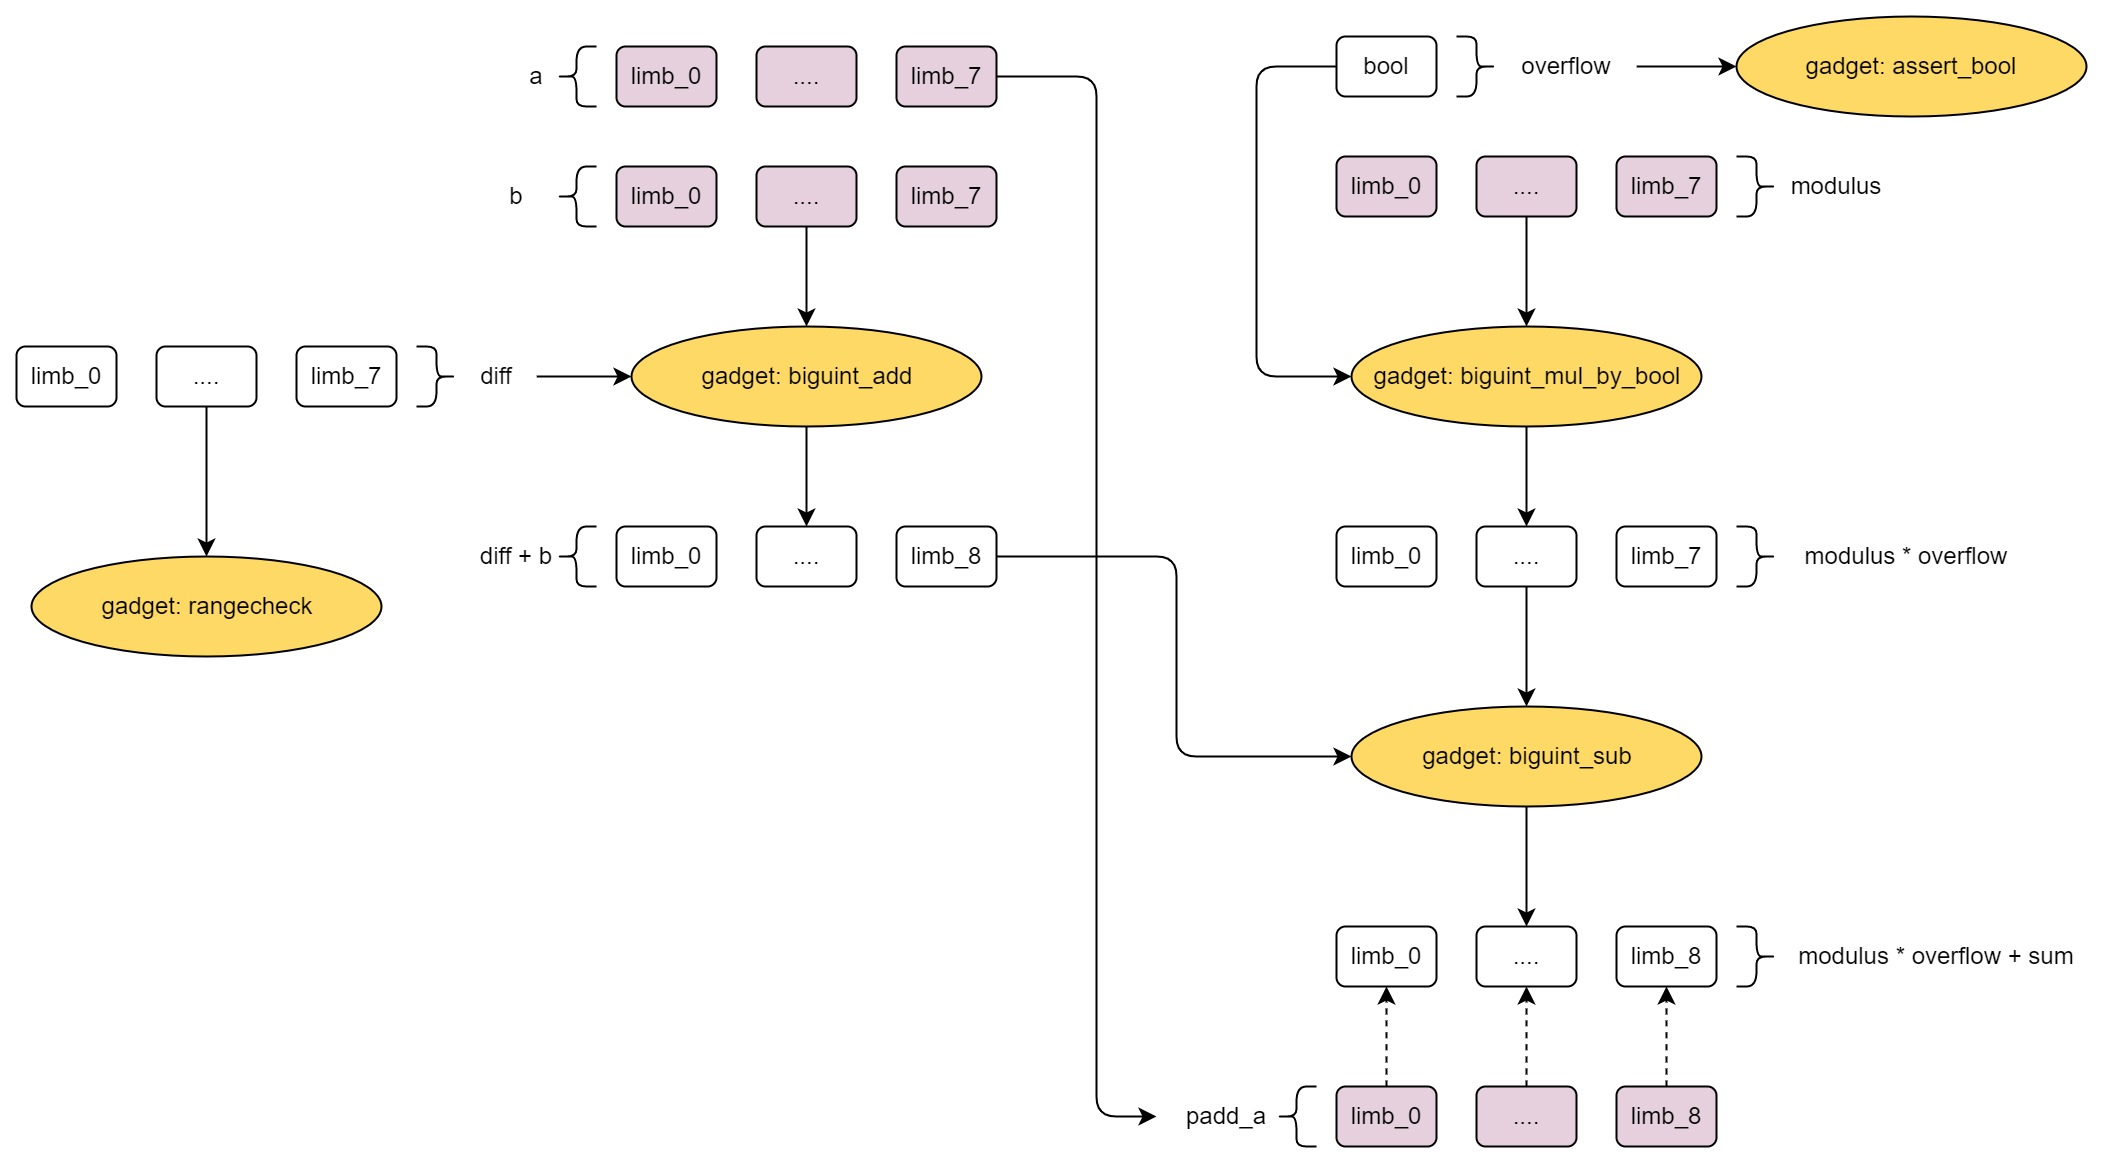
\includegraphics[width=0.6\textwidth]{nonnative-sub-layout.jpg}
    \caption{non-native-sub layout}
    \label{fig:non-native-sub-layout}
\end{figure}